\documentclass{article}

% Language setting
% Replace `english' with e.g. `spanish' to change the document language
\usepackage[english]{babel}

% Set page size and margins
% Replace `letterpaper' with`a4paper' for UK/EU standard size
\usepackage[letterpaper,top=2cm,bottom=2cm,left=3cm,right=3cm,marginparwidth=1.75cm]{geometry}

% Useful packages
\usepackage{amsmath}
\usepackage{graphicx}
\usepackage[colorlinks=true, allcolors=blue]{hyperref}
\usepackage[section]{placeins}
\graphicspath{
    {../plots}
}

\title{Supervised Learning with Movies and Credit}
\author{Josh Gillette}
\date{February 11, 2024}

\begin{document}
\maketitle

\section{Introduction}

This paper will analyze multiple supervised learning algorithms through two diverse classification problems. The first of which will attempt to predict whether a movie will have a high popularity score based on several release criteria. The second problem will aim to determine whether a borrower will default on their debt.

These problems are especially interesting with respect to one another as the movies dataset is smaller (5 features, $\sim5,400$ rows) and was heavily preprocessed. The data was directly pulled from The Movie Database and the features and label were selected only by intuition. On the other hand, the credit card dataset is extremely large (24 features, 30,000 rows) and represents a more conventional classification problem that was externally composed.

These differences in datasets will provide unique opportunities to compare and tune various supervised learning algorithms.

\section{The Problems}

\subsection{Movies}

Following a movie's theatrical run, it will eventually get a home release. This could encompass various distribution channels such as a physical purchase (tape, DVD, Blue-ray), digital purchase, television broadcasts, or streaming. For obvious reasons, the overseers of any of these distribution channels would be interested in acquiring the most popular movies. For example, a streaming service exclusively offering a movie to attract more subscribers.

Using The Movie Database, or TMDB, data was aggregated with the following features:
\begin{itemize}
    \item runtime: how long the movie is in minutes
    \item release\_year: the movie's year of release
    \item is\_franchise: whether the movie belongs within a franchise (i.e Avengers is in the Marvel franchise)
    \item budget: how much it cost (in USD) to make the movie
    \item revenue: how much (in USD) the movie made
    \item is\_popular (y): whether a movie is one standard deviation $(\sim 8.5)$ above the average popularity value $(\sim 9.5)$. In other words if a movie's popularity $>18$.
\end{itemize}
This problem is interesting for a couple reasons. As mentioned, it is not only a relatively smaller dataset in both features and size, but its features and label were custom selected from a larger, 23 featured dataset so clear results are not guaranteed.

Another interesting aspect of this data is how intertwined the features are with one another, and how they each translate to popularity. For instance movie runtimes that are too long tend to be less popular. Or a movie's release year informs how that movie is distributed and consumed, as the data includes movies released from 1915 (well before the TV was invented) to 2017 (where movies are increasingly being consumed on non-TV devices). Budget and revenue also do not have a direct effect on popularity as low budget movies can become extremely popular (Rocky) as well as low revenue movies (The Shawshank Redemption). Lastly, movie franchises seemingly garner immense popularity, but this may be dependent on release year and budget.

This classification problem is clearly interesting due to its limited relative size as well as the relationship the features have with one another.

\subsection{Credit}

Credit companies loan funds to a customer in expectation that the loan amount will be repaid at the end of the month. Failing to repay the loan amount will result in the customer accruing interest, and if failure to repay continues, the customer will default on those loans. This results in the credit company often closing the account (and losing the customer), as well as pursue costly debt collection actions. It is clearly in the credit companies interest to predict if a customer is about to default so action can be taken.

A dataset was obtained that represents Taiwanese customers' credit data and whether they ultimately defaulted. This dataset contains the following 24 features:
\begin{itemize}
    \item credit\_limit: credit limit
    \item sex: sex (male/female)
    \item education: education (graduate school, university, high school, other)
    \item marriage: marriage status (married, single, other)
    \item age: age (years)
    \item payment\_history (7 months): (repayment status, bill statement amount, amount paid)
    \item defaulted: whether they defaulted
\end{itemize}

This problem is interesting in and of itself, but also in contrast to the movies dataset. Outside of the 21 features attributed to payment history, each feature is more independent to one another compared to the movie dataset. Although there are social correlations that link features like education, marriage, and age, this is much less prevalent than in the movies database. The payment history features which include the repayment status, bill statement amount, and amount paid for seven contiguous months also provides an interesting aspect of this data.

Additionally, the size of the credit dataset is much larger than the movies dataset. The number of features ($\sim 5x$ the movies dataset) and size (also $\sim 5x$ the movies dataset). This not only provides more data, but also may impact the way that the learning algorithms are tuned and optimized. The credit dataset may offer a more conventional example of learning data, but has certain nuances and will be valuable in juxtaposition of the movies dataset.

\pagebreak
\section{Learning}

\subsection{Decision Trees}

Decision trees utilize a tree-like structure to create and evaluate decision rules that are derived from the the data's features. The implemented decision tree utilizes some minor pre-pruning methods. Namely, limiting the max\_depth to 8 for both data sets, and setting min\_samples\_split to 10 for just the credit dataset.
\subsubsection{Varied train size}

\begin{center}
    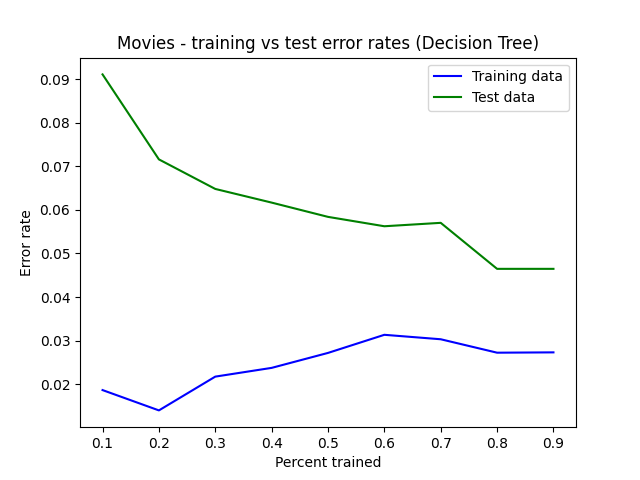
\includegraphics[width=.45\linewidth]{movies-decision_tree-error.png}
    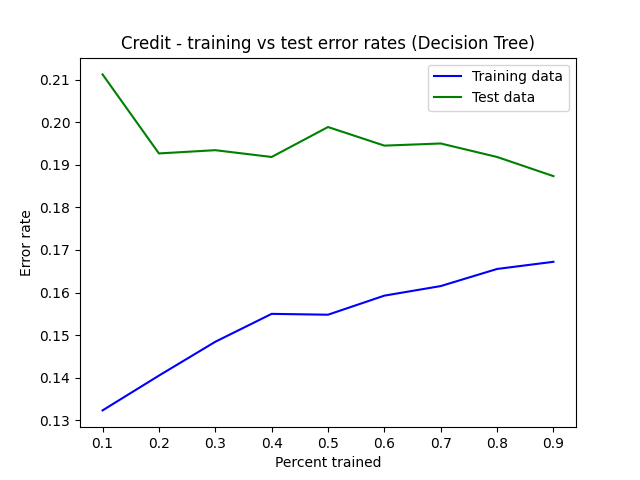
\includegraphics[width=.45\linewidth]{credit-decision_tree-error.png}
\end{center}

Both datasets benefited from an increase in training data, as the test data reported lower error rates.
The increase in training data error can be attributed to the setting of max\_depth, which avoids overtraining and produces a smaller clock time (see Appendix), which ultimately benefits the test data. Decision trees yielded an error rate of 0.05 for the movies dataset, and 0.19 for the credit dataset.
\subsubsection{Varied max\_depth (hyperparameter)}

\begin{center}
    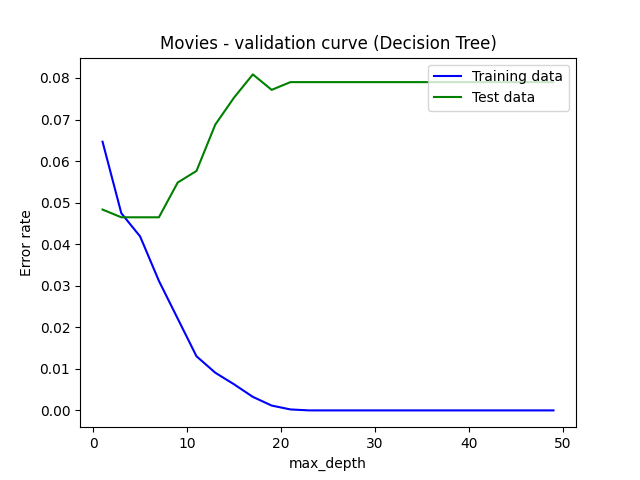
\includegraphics[width=.45\linewidth]{movies-decision_tree-validation_curve.png}
    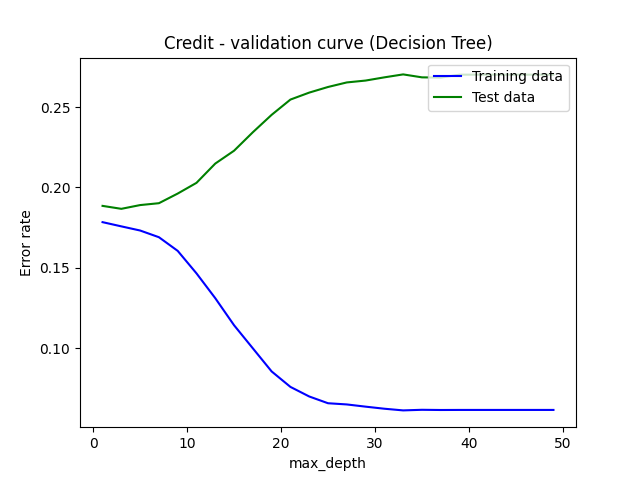
\includegraphics[width=.45\linewidth]{credit-decision_tree-validation_curve.png}
\end{center}

The above conveys the damage that a high tree depth can do. The tree becomes overfitted to the training data, and an inverse relationship between the training and test data emerge. For both the movies and credit datasets, the error rate is increased as max\_depth increases past $\sim 8$.
\subsection{Neural Networks}

Neural networks utilize deep learning and and interconnected network of nodes that inspired by biological neural paths. This implementation of neural networks was fairly standard with the activation function set to relu and solver set to lbfgs. The net's hidden layers were set to include just a single hidden layer, each with 3 hidden units, which proved effective and resource efficient.

\subsubsection{Varied train size}

\begin{center}
    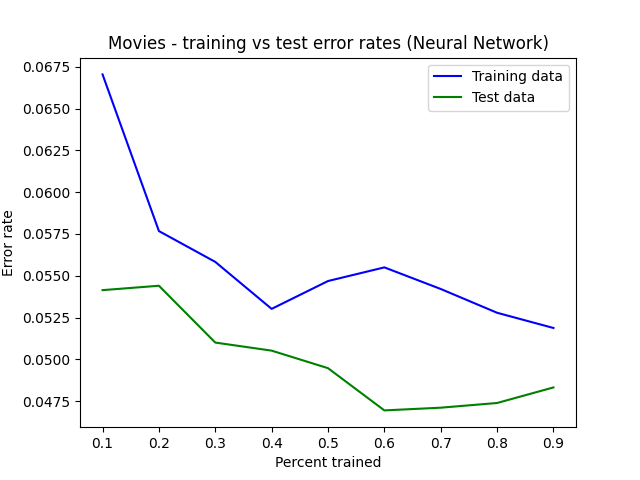
\includegraphics[width=.45\linewidth]{movies-neural_net-error.png}
    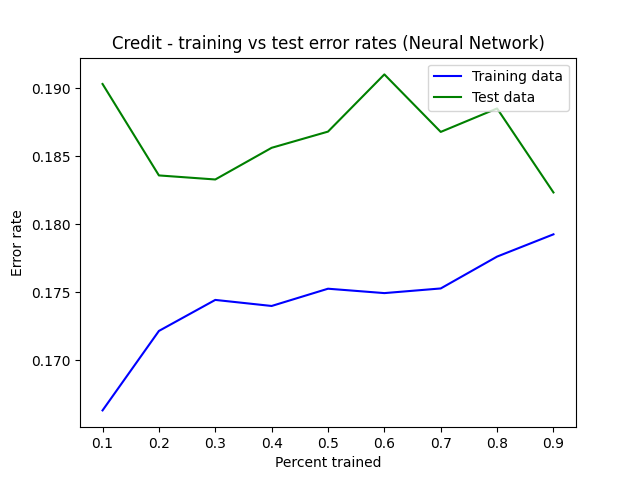
\includegraphics[width=.45\linewidth]{credit-neural_net-error.png}
\end{center}

For the movies dataset, the error rate of both the training and test dataset decrease as more data is trained on. As for the credit dataset, test data error rates remain roughly the same with more training data, but begins to decrease with a majority training dataset. The test error rate for the movies dataset settles at 0.05, and 0.19 for the credit dataset.
\subsubsection{Varied hidden layers (hyperparameter)}

\begin{center}
    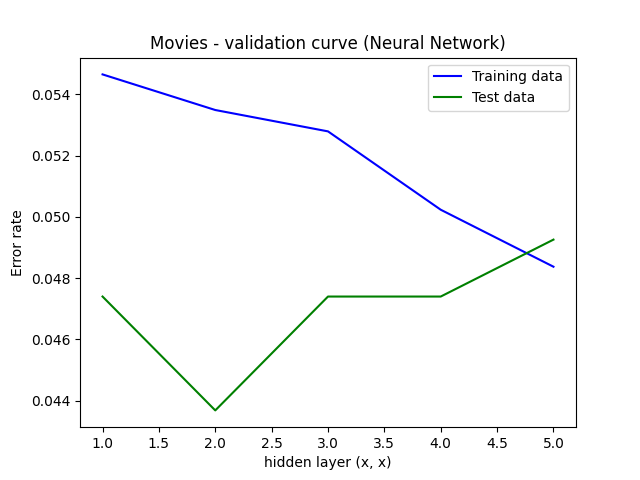
\includegraphics[width=.45\linewidth]{movies-neural_net-validation_curve.png}
    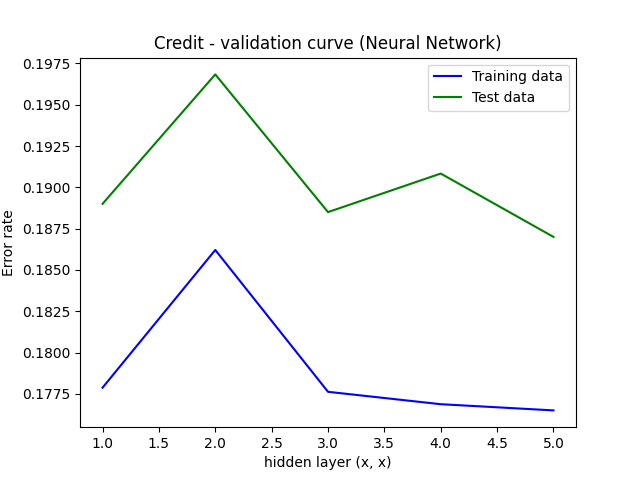
\includegraphics[width=.45\linewidth]{credit-neural_net-validation_curve.png}
\end{center}

As the neural net's single hidden layer's hidden units are increased, the training error rate decreases, while the test data set increases for the movies dataset and decreases for the credit dataset. This, in addition to the increase wall clock time (see Appendix) or training more hidden layers/units, led to the universal selection of a single hidden layer with 3 hidden units.

\subsection{Boosted Decision Trees}

Boosted decision trees combines many potentially weak learners to effectively classify data. This Boosting configuration uses a similar max\_depth from standard decision trees from above at 9, and sets the number of boosting stages to 25. Learning rate is set constant to 1.
\subsubsection{Varied train size}

\begin{center}
    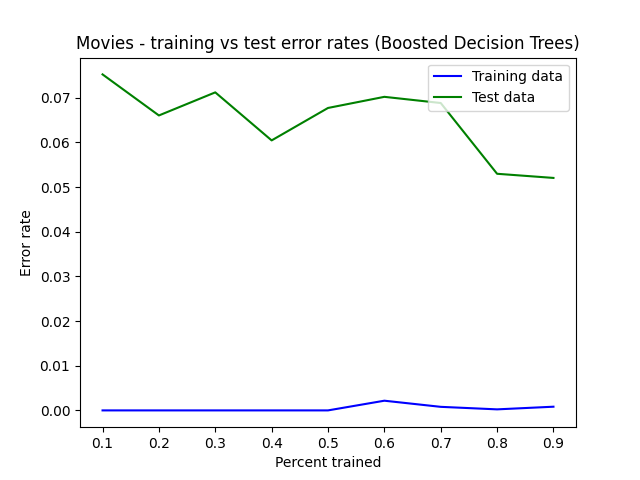
\includegraphics[width=.45\linewidth]{movies-boosted-error.png}
    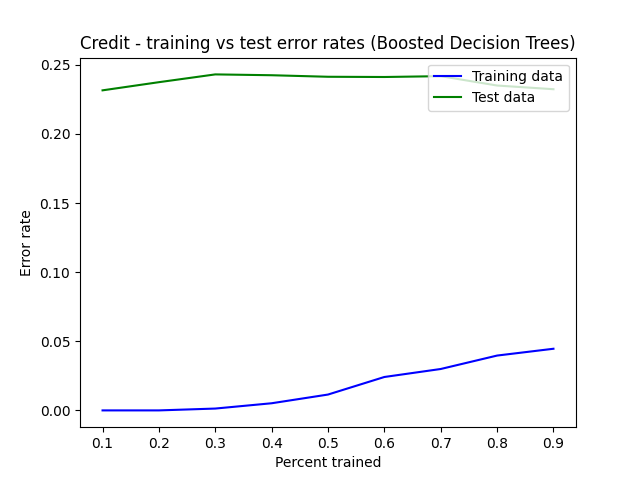
\includegraphics[width=.45\linewidth]{credit-boosted-error.png}
\end{center}

This classifier sees very low training data error rates, and performance in test data error rates decrease with training data on the movies dataset, and result in little change on the credit database. The movies dataset sees an error rate of about 0.05, and 0.24 for the credit dataset.

\subsubsection{Varied n-estimators (hyperparameter)}

\begin{center}
    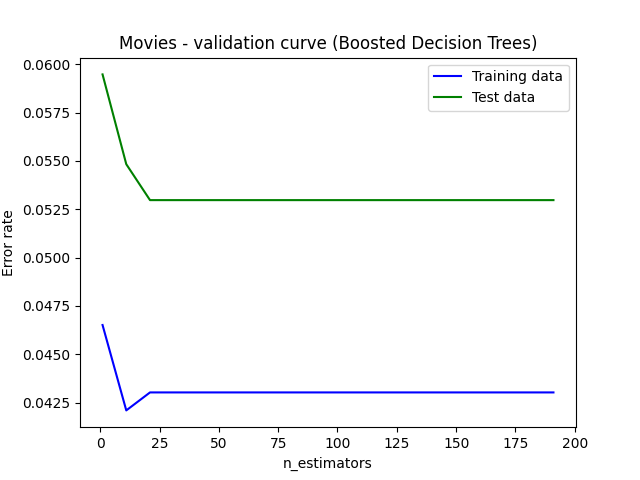
\includegraphics[width=.45\linewidth]{movies-boosted-validation_curve.png}
    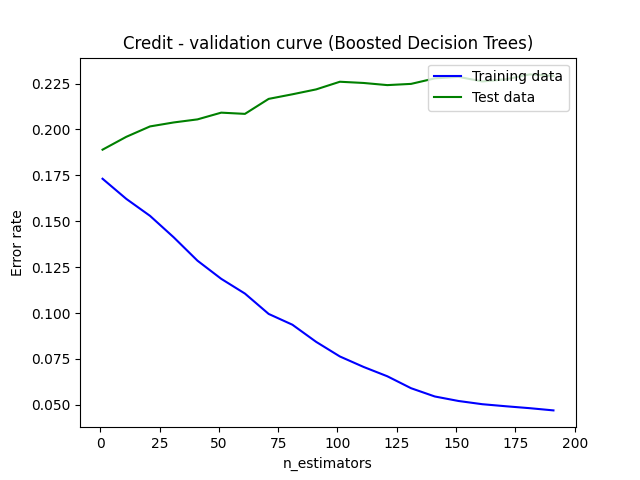
\includegraphics[width=.45\linewidth]{credit-boosted-validation_curve.png}
\end{center}

Inspecting the n\_estimators or boosting stages value for the movies dataset, it can be clearly seen that there is no improvement after $\sup 25$. However, for the credit dataset the number of boosting stages results in worse test data performance, and eventual overfitting. This again supports a lower boosting stages value.

\subsection{Support Vector Machines (SVM)}

Support vector machine or SVMs are supervised max-margin models. This SVM implementation uses the stock 'rbf' kernel, with no other notable mention

\subsubsection{Varied train size}

\begin{center}
    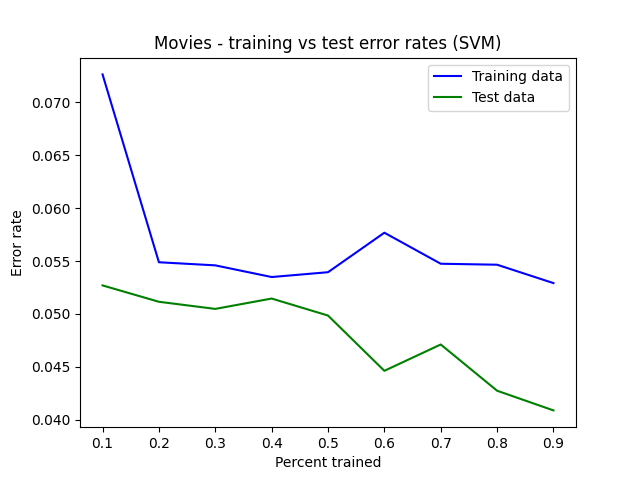
\includegraphics[width=.45\linewidth]{movies-svc-error.png}
    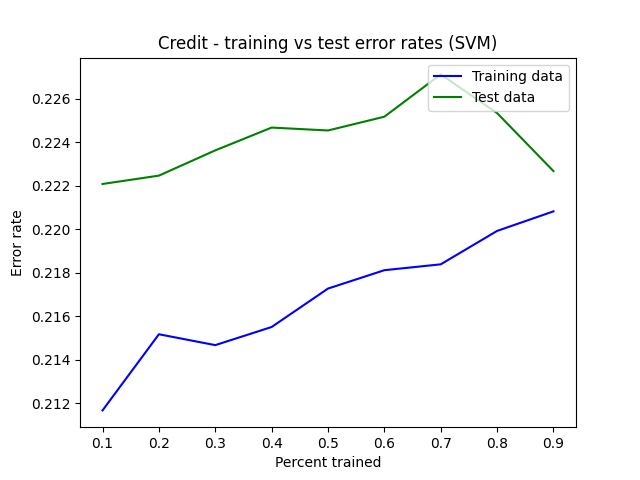
\includegraphics[width=.45\linewidth]{credit-svc-error.png}
\end{center}

As was the case in both neural networks and decision trees, SVM results in the two datasets trending in opposite directions as more data is trained on. The movies dataset seeing a general decrease in error rates, while the credit dataset sees an increase in error rate. Both datasets see a general convergence of training and test data error rates. The movies dataset yields a 0.04 error rate and 0.22 for the credit dataset.

\subsubsection{Varied kernel (hyperparameter)}

\begin{center}
    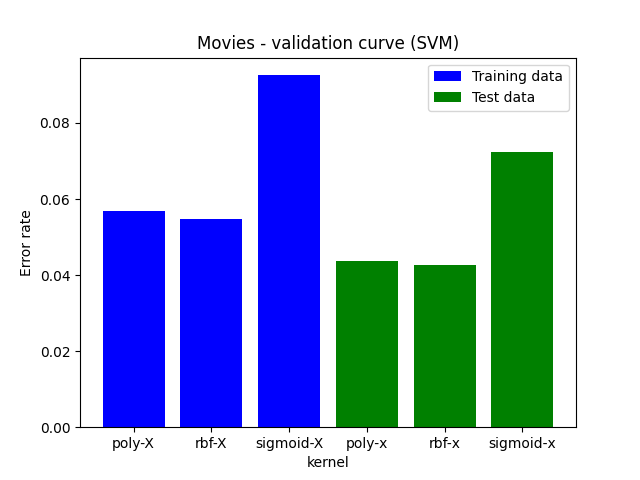
\includegraphics[width=.45\linewidth]{movies-svc-validation_curve.png}
    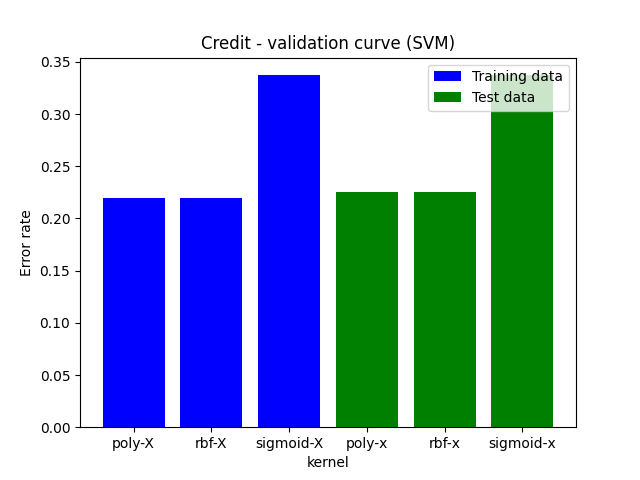
\includegraphics[width=.45\linewidth]{credit-svc-validation_curve.png}
\end{center}

Outside of the sigmoid kernel which results in increased error rates, modifying the other kernels (poly, rbf) does not see a major change in error rate for both datasets. However, the poly kernel takes significantly longer to complete than the rbf kernel.

\subsection{k-Nearest Neighbors}

The k-nearest neighbors method uses data proximity to make predictions a set of data points. This KNN implementation was modified to set the number of default neighbors to 4.

\subsubsection{Varied train size}

\begin{center}
    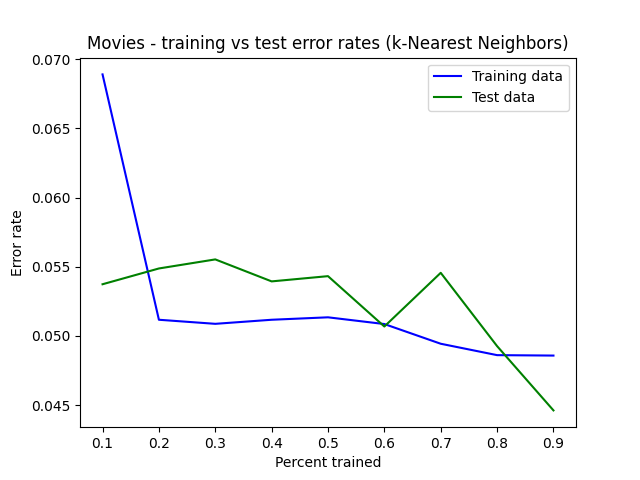
\includegraphics[width=.45\linewidth]{movies-k_nearest-error.png}
    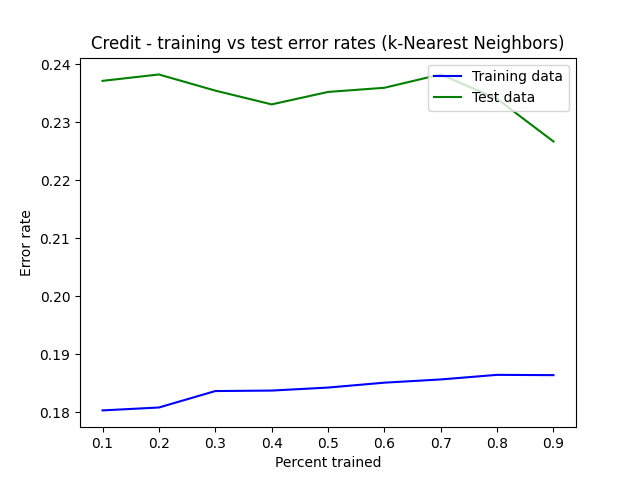
\includegraphics[width=.45\linewidth]{credit-k_nearest-error.png}
\end{center}

In both datasets, the more data that is trained on results in a lower, or similar, error rate. The movies dataset produces a 0.05 error rate while the credit dataset produces a 0.23 error rate.

\subsubsection{Varied n-neighbors (hyperparameter)}

\begin{center}
    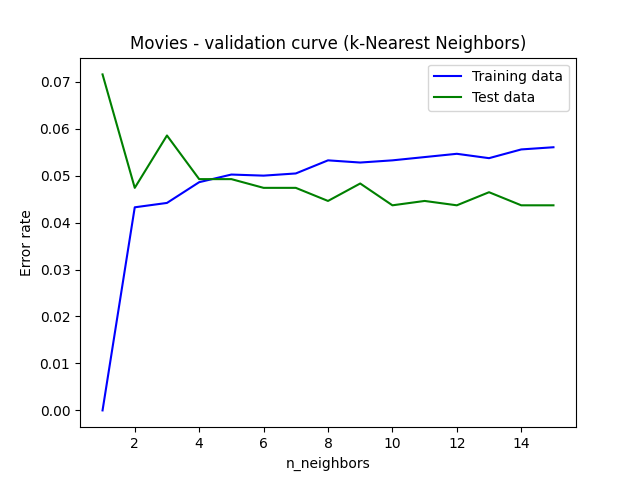
\includegraphics[width=.45\linewidth]{movies-k_nearest-validation_curve.png}
    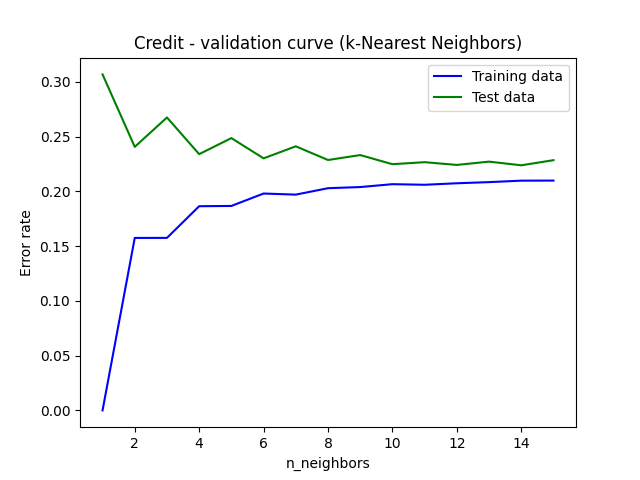
\includegraphics[width=.45\linewidth]{credit-k_nearest-validation_curve.png}
\end{center}

The above supports the reasoning for seeing the default number of neighbors to use to 4, as error rates are not significantly decreases for the potential increase to wall clock time (see Appendix).

\pagebreak

\section{Analysis}

The results, with respect to each classification problem, are very consistent between each learning algorithm. Error rates at $\sup80\%$ training for the test data hover in the 0.04-0.05 range for the movies dataset, and 0.19-0.23 for the credit dataset. Differently put, the learning models are able to predict a movie's popularity with $\sup 95\%$ success rate, and whether an individual will default on their debt with $\sup 80\%$ probability. By this, it can be concluded that the nature of the datasets may be more important the the algorithm performance themselves. Performance from technique to technique within a dataset produced significantly more similar results than when comparing two datasets within the same technique.

To highlight a couple techniques, the decision tree classifier performed extremely well when comparing its total runtime, however it requires a larger share of training data to see this performance. With respect to sole performance, neural nets provided the best error rates and stayed fairly consistent when faced with lower training data.

Overall, these supervision techniques prove to be robust with respect to the amount of trained data as well as hyperparameters. For example, when these models have access to less than 80\% training data, they still prove to be reliable with predictions. These results, the models being so consistent among and within one another, is likely due to both datasets having extensive and unique data that represents the problem space well. The movies dataset performed especially well as it contained few features, but those features were again well represented with a diverse set of inputs of varying combination, which is foundational for a learning algorithm to train on.

Although performance among the algorithm's results were similar, one thing that was not was wall clock time, or simply the amount of time each algorithm took to run on a personal machine. Looking at the credit dataset, the decision tree classifier was able to complete in a third of a second at 80\% training data, while SVC with the poly kernel took 20-30 minutes. Despite the time difference, the results for these two supervision techniques were very similar. Fortunately, most methods did not see any non-linear increase as training data or hyperparameters were increased. Further, these algorithms likely had difference space complexities that was not measured in this report.

Observing the very similar performance, some not yet understood relationships between the training and test data between techniques, and the wide ranging runtimes, it appears that more time could be spent in tuning each technique and algorithm. For example the neural net's solver, the boosting's learning rate, and SVC's kernel type (although this one proved to be very resource heavy). The results of tuning each of these algorithms was not always intuitive, especially as how these tunings related to the training data error rates.

In conclusion, these various supervision techniques outline the data-driven nature of machine learning. A major aspect of selecting and using certain techniques is not just about minimizing error rate, but also consists of finding the most efficient methods with respect to both required data, time, and space.

\pagebreak

\appendix
\section{Appendix (wall clock times, credit dataset)}
\begin{center}
    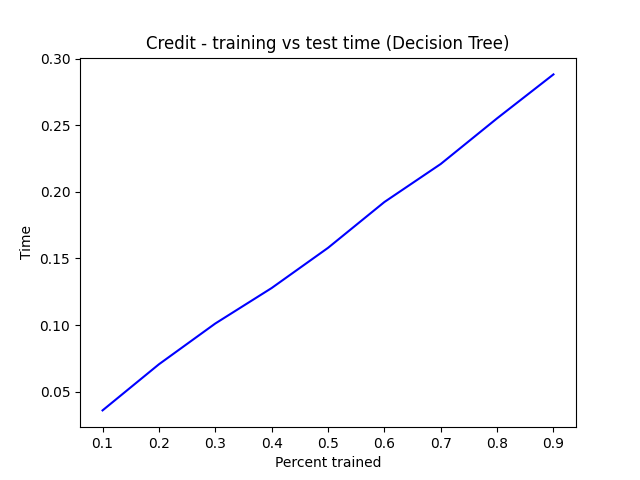
\includegraphics[width=.45\linewidth]{credit-decision_tree-error-time.png}
    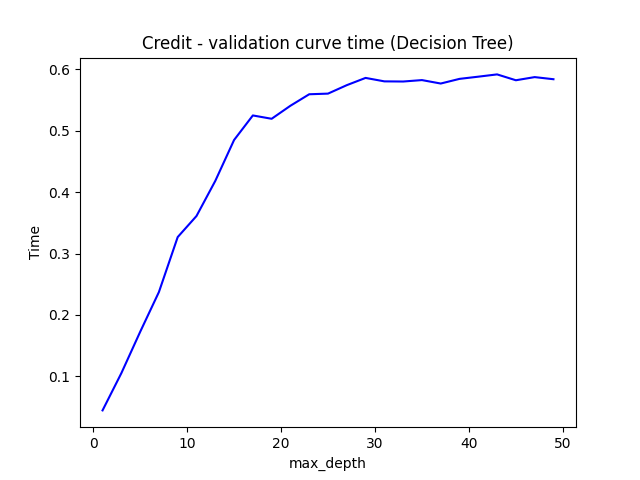
\includegraphics[width=.45\linewidth]{credit-decision_tree-validation_curve-time.png}
    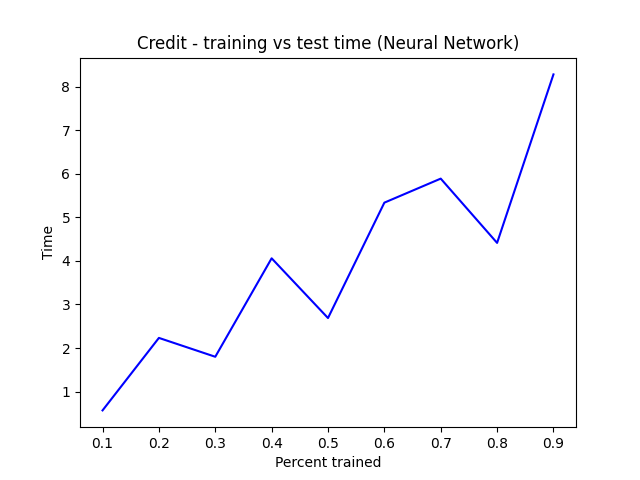
\includegraphics[width=.45\linewidth]{credit-neural_net-error-time.png}
    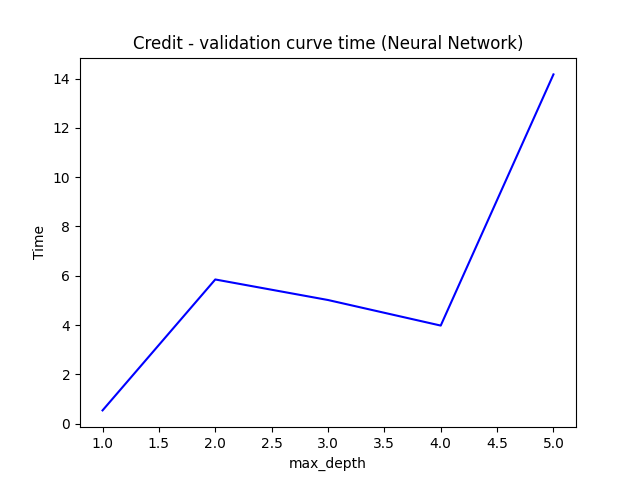
\includegraphics[width=.45\linewidth]{credit-neural_net-validation_curve-time.png}
    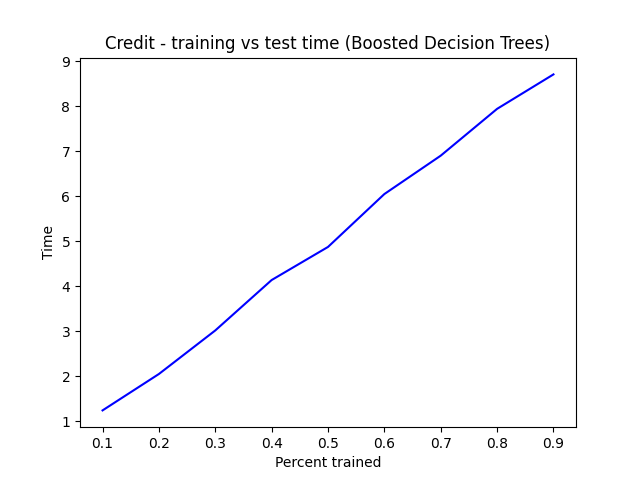
\includegraphics[width=.45\linewidth]{credit-boosted-error-time.png}
    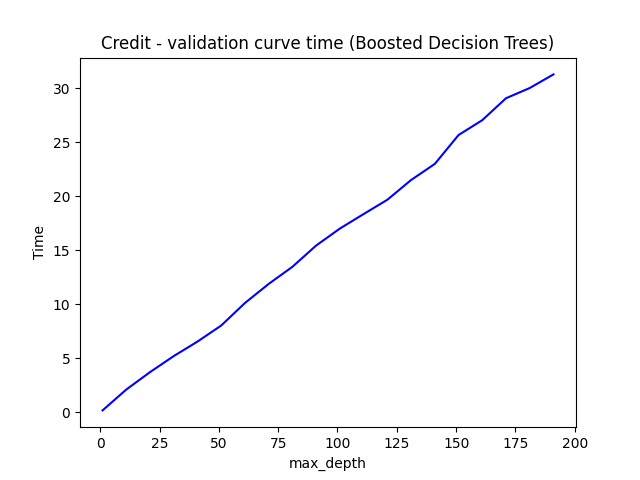
\includegraphics[width=.45\linewidth]{credit-boosted-validation_curve-time.png}
    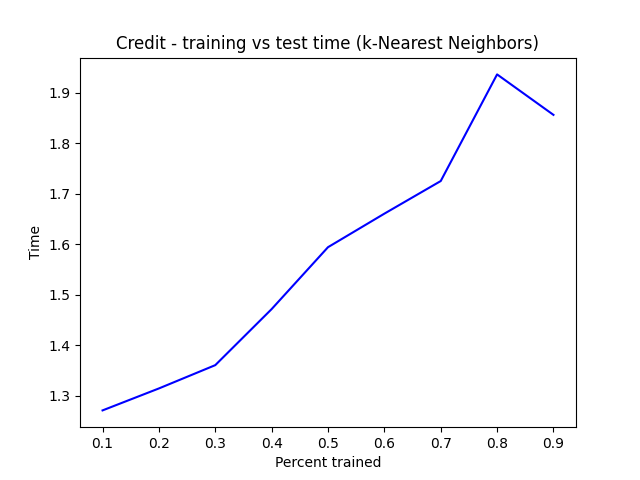
\includegraphics[width=.45\linewidth]{credit-k_nearest-error-time.png}
    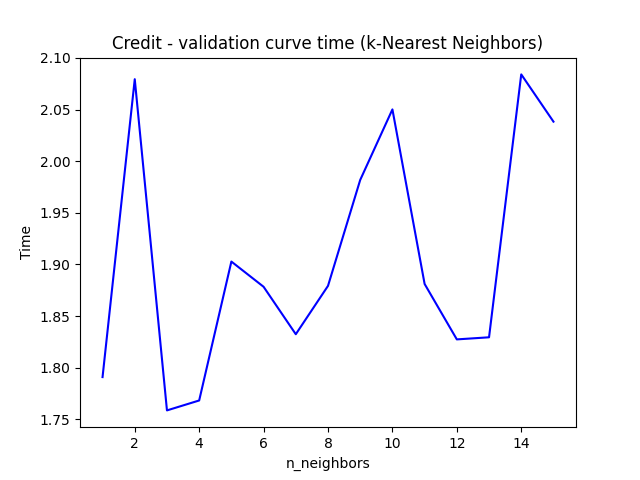
\includegraphics[width=.45\linewidth]{credit-k_nearest-validation_curve-time.png}
\end{center}

\pagebreak
\bibliographystyle{alpha}
\bibliography{sample}

Quinlan,Ross. Statlog (Australian Credit Approval). UCI Machine Learning Repository.\\ https://doi.org/10.24432/C59012.

\end{document}
